\section{Stacks and Heaps}
\label{sec:stacks_heaps}

\noindent
To further understand how our algorithms run, we must understand ligtly how memory is passed around in our programs.

\begin{Def}[Machine Code \& Compilation]

    \label{def:machine_code}

    Code is separated into two main areas of memory management, the program itself, and the data in transit during execution.
    The program itself is broken up such as follows:
    \begin{itemize}
        \item \textbf{Text Segment:} The part of the program which contains the executable code.
        \item \textbf{Data Segment:} The part of the program which contains global and static variables.
        \item \textbf{Machine Code:} The compiled code of the program, which is executed by the CPU.
    \end{itemize}

    \noindent
    Once the code compiles, we our data segment is further divided into two parts in memory:
    \begin{itemize}
        \item \textbf{Initialized Data:} This is data that has been given a value before the program starts running, such as global variables.
        \item \textbf{Uninitialized Data:} This is data that has not been given a value before the program starts running, such as local variables.
    \end{itemize}
    \noindent
    By memory we mean the \textbf{RAM (Random Access Memory)} hardware component, which stores temporary data, constantly 
    communicating with the CPU or external storage (e.g., hard drive, SSD).
\end{Def}

\noindent
Let's talk about our first data structure, the stack:
\begin{Def}[Stack]

    A \textbf{stack data structure} is a collection of elements that follows a \textbf{Last In, First Out} (LIFO) principle. I.e., in a 
    stack of plates, the last added plate is the first one to be removed, not the middle or bottom/first plate.
    Each \textit{plate} in the stack is called a \textbf{stack frame}.
\end{Def}

\newpage

\noindent
This text does not concern assembly code or low-level programmming, so \underline{\textbf{do not}} get caught up on the specifics of this next example:
\begin{Example}[Assembly Code]

    \label{ex:assembly_code}
    Here is an assembly code example that demonstrates both initialized and uninitialized data. 
    Initialized data is placed in the `.data` section, while uninitialized data is placed in the `.bss` section:

    \begin{lstlisting}[language={[x86masm]Assembler}, numbers=none]
    section .data               ; Initialized data section
        num1    dd  7           ; num1 is initialized to 7
        num2    dd  3           ; num2 is initialized to 3

    section .bss                ; Uninitialized data section
        temp    resd 1          ; temp is reserved (uninitialized)
        result  resd 1          ; result is reserved (uninitialized)

    section .text               ; Code section
        global _start

    _start:
        mov eax, [num1]         ; Load num1 into eax
        mov [temp], eax         ; Store num1 in temp
        mov ebx, [num2]         ; Load num2 into ebx
        add eax, ebx            ; Add num2 to eax (eax = num1 + num2)
        mov [result], eax       ; Store the sum in result
    ; (Exit code omitted for brevity)
    \end{lstlisting}

    \noindent
    In this example, `num1` and `num2` are initialized before execution, while `temp` and `result` are uninitialized and only receive values during program execution.
\end{Example}

\noindent
Now let's look at how our programs utilize the stack:
\begin{Def}[Call Stack]

    A \textbf{call stack} is a stack which keeps track of function calls in a program as well as any local variables within such functions.
    
    \underline{This is why we say a variable is in \textbf{scope}}, as when a function is taken off the stack, or a new stack frame 
    is placed ontop, the variables in the previous or discarded stack frame are \textbf{no longer accessible}.
\end{Def}

\newpage 

\noindent
Let's illstrate this with the following diagram:

\begin{figure}[h]
    \centering
    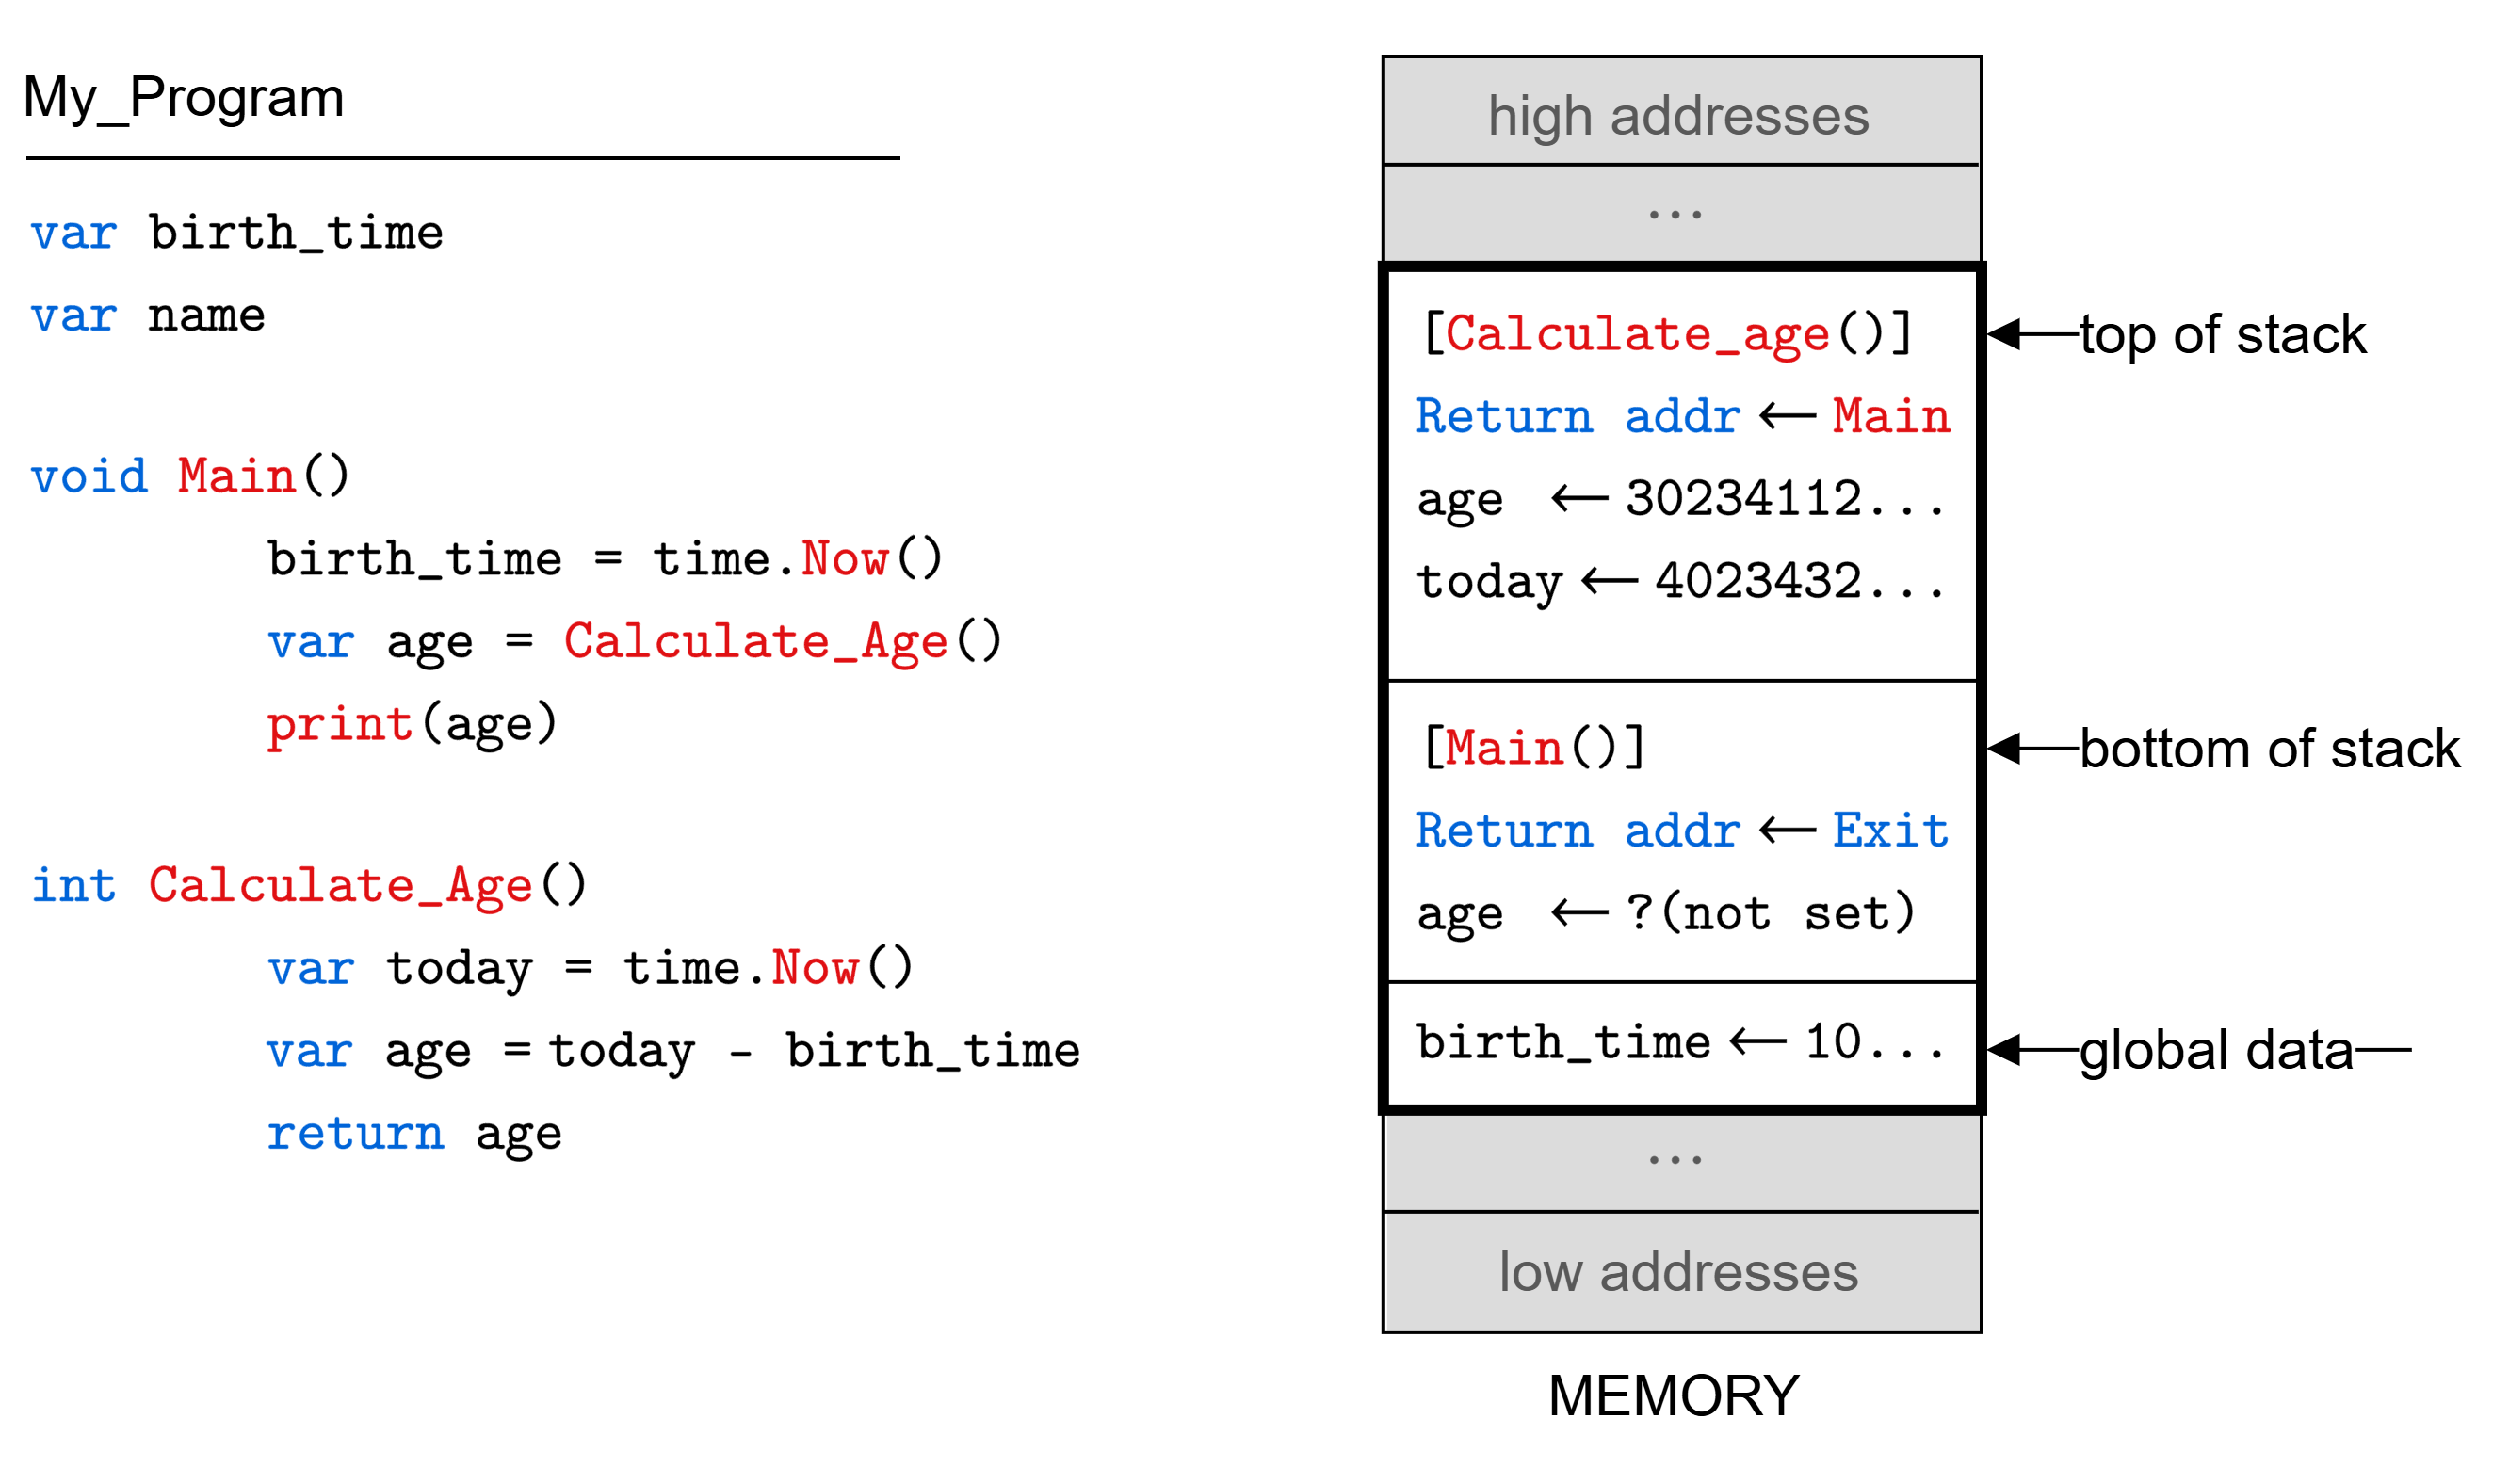
\includegraphics[width=0.8\textwidth]{./Sections/stacks_heaps/call_stack.png}
    \caption{Here is a simplified look at how memory manages the stack. On the left is our program written 
    in some abstract language, and on the right is the call stack in memory (simplified). 
    The program has a global `birth\_time' variable, which is intialized in the \texttt{Main} function. The \texttt{Main} function
    then calls the \texttt{Calculate\_Age} function which uses the `birth\_time' variable to calculate the `age' via the difference of 
    the current time and the `birth\_time.'
    Lookin at the memory, we see at the bottom of our memory contains global variables accessible to any frame. Next, is the bottom of the stack, containing a return address to exit 
    the program, while awaiting the result of the function call for `age'. The top of our stack contains another frame that we will return the value
    a new `age' (not the same as the one before) not accessible from the main function. This new frame also contains a new local variable `today.'
    Once this function returns, \texttt{Main} will have the result of its local variable `age.'. Concretely, the 
    `age' variable in both the \texttt{Main} and \texttt{Calculate\_Age} function are completely separate despite sharing the same \textit{name}.}
    \label{fig:call_stack}
\end{figure}

\noindent
\rule{\textwidth}{0.4pt}\\

\noindent
\underline{\textbf{Please Note:} The above figure is a simplified version}; This presentation derivatives from what actually happens
for teaching sake. In the following pages we define the stack frame in more detail.

\begin{Tip}
A lot of demonstrations (including this text) will show the stack growing \textbf{upwards}; This is strictly because it's easier to visualize and does not
accurately potray what a stack really does or looks like. In the following pages we will clear this up, and show how the stack actually grows from top-to-bottom.
Of course, there is always room for deviation if a developer wishes to implement a stack in some other arbitrary way. Nonetheless, the following is what one 
might typically expect in a stack implementation.
\end{Tip}

\newpage 
\begin{Def}[Instructions]

    The CPU register (IP/EIP) is the \textbf{instruction pointer}, pointing to the next opreation to execute. All commands are baked 
    into the CPU; This includes the \textbf{ALU (Arithmetic Logic Unit)}, \textbf{Memory Unit (load/store)}, and \textbf{Control Unit (branching/looping)}.
    All instructions are given a numeric ID called an \textbf{opcode} (operation code). 
    
    The CPU fetches the instruction from memory, decodes it, and executes it. This process is repeated until the program terminates.
    Languages like assembly interface this with human-readable mnemonics, such as `MOV', `ADD', `SUB', etc (as seen in Example \ref{ex:assembly_code}).
    
\end{Def}
\begin{Def}[Stack Frame Anatomy]

Under the x86-32 calling convention Two registers keep track our place in the stack:
\begin{itemize}
  \item \textbf{Base Pointer (BP/EBP):} Points to the base (i.e.\ ``bottom'') of the current function's stack frame.
  \item \textbf{Stack Pointer (SP/ESP):} Points to the ``top'' of the current function's stack frame, i.e., the next free byte where a push would land.
\end{itemize}

\noindent
When the program starts, the operating system \emph{reserves} a contiguous region of memory for the stack. By convention, the \emph{bottom} of that region lies at a higher address, 
and the stack ``grows downward'' toward lower addresses as data is pushed. If the stack pointer ever moves past the reserved limit---a \textbf{stack overflow} occurs.
\\

\noindent
A single \textbf{stack frame} itself is a contiguous block of memory in which the function stores:
\begin{itemize}
  \item \textbf{Parameters:} The arguments passed in by the caller,  
  \item \textbf{Return Address:} The address of the next instruction to execute after the function returns,
  \item \textbf{Old Base Pointer:} The caller's `EBP', saved so that on return we can restore the previous frame,
  \item \textbf{Local Variables:} Space for any locals or temporaries that the function needs.  
\end{itemize}

\noindent
This is why variables in previous or new functions calls become ``\textbf{out of scope}'' (no longer accessible), as they belong to some other stack frame; 
When it comes to \textbf{Global Variables}, they live in a separate region of memory, defined by the \textbf{data segment} (\ref{def:machine_code}).

Moreover, a call to a new function invokes the \underline{\textbf{call} instruction}, this automically pushes the return address to the current frame onto the stack.
Additonally, the CPU reserves the \textbf{EAX} register for the return value (number or address) of a function. 
When the function returns, it can place its result in `EAX', and the caller can retrieve it from there. During constant use 
the `EAX' \underline{register may contain \textbf{garbage}} data from previous use, unless explicitly set to zero or some other value.
\end{Def}

\newpage 

\begin{table}[h]
\centering
\resizebox{\textwidth}{!}{
\begin{tabular}{|c|c|l|}
\hline
\multicolumn{3}{|c|}{\textbf{High Addresses}} \\ \hline
\textbf{Contents}       & \textbf{Offset} & \textbf{Notes} \\
\hline
\emph{(Parameters 3, 4, \(\dots\))} & \(\mathit{EBP} + 16\), \(+20\), \(\dots\) & Third-and-onward arguments, if any. \\ 
Parameter 2            & \(\mathit{EBP} + 12\) & Second argument passed on stack. \\
Parameter 1            & \(\mathit{EBP} + 8\)  & First argument passed on stack. \\
Return Address         & \(\mathit{EBP} + 4\)  & Auto-pushed by the \texttt{call} instruction.\\
Old EBP (Saved BP)     & \(\mathit{EBP} + 0\)  & The caller's base pointer \\
\hline
\multicolumn{3}{|c|}{\textbf{Current Frame (locals/temporaries)}} \\ \hline
Local Variable 1        & \(\mathit{EBP} - 4\)  & First 4-byte local (or smallest slot). \\
Local Variable 2        & \(\mathit{EBP} - 8\)  & Next 4-byte local or part of a larger object. \\
\(\dots\)                      & \( \vdots \)         &(additional locals at \(\mathit{EBP} - 12,\ -16,\ \dots\)) \\
\hline
\multicolumn{3}{|c|}{\textbf{Low Addresses}} \\ \hline
\end{tabular}
}
\caption{Typical x86-32 Stack-Frame Layout, where offsets are typically a multiple of 4 bytes.}
\end{table}

\begin{figure}[!ht]
    \centering
    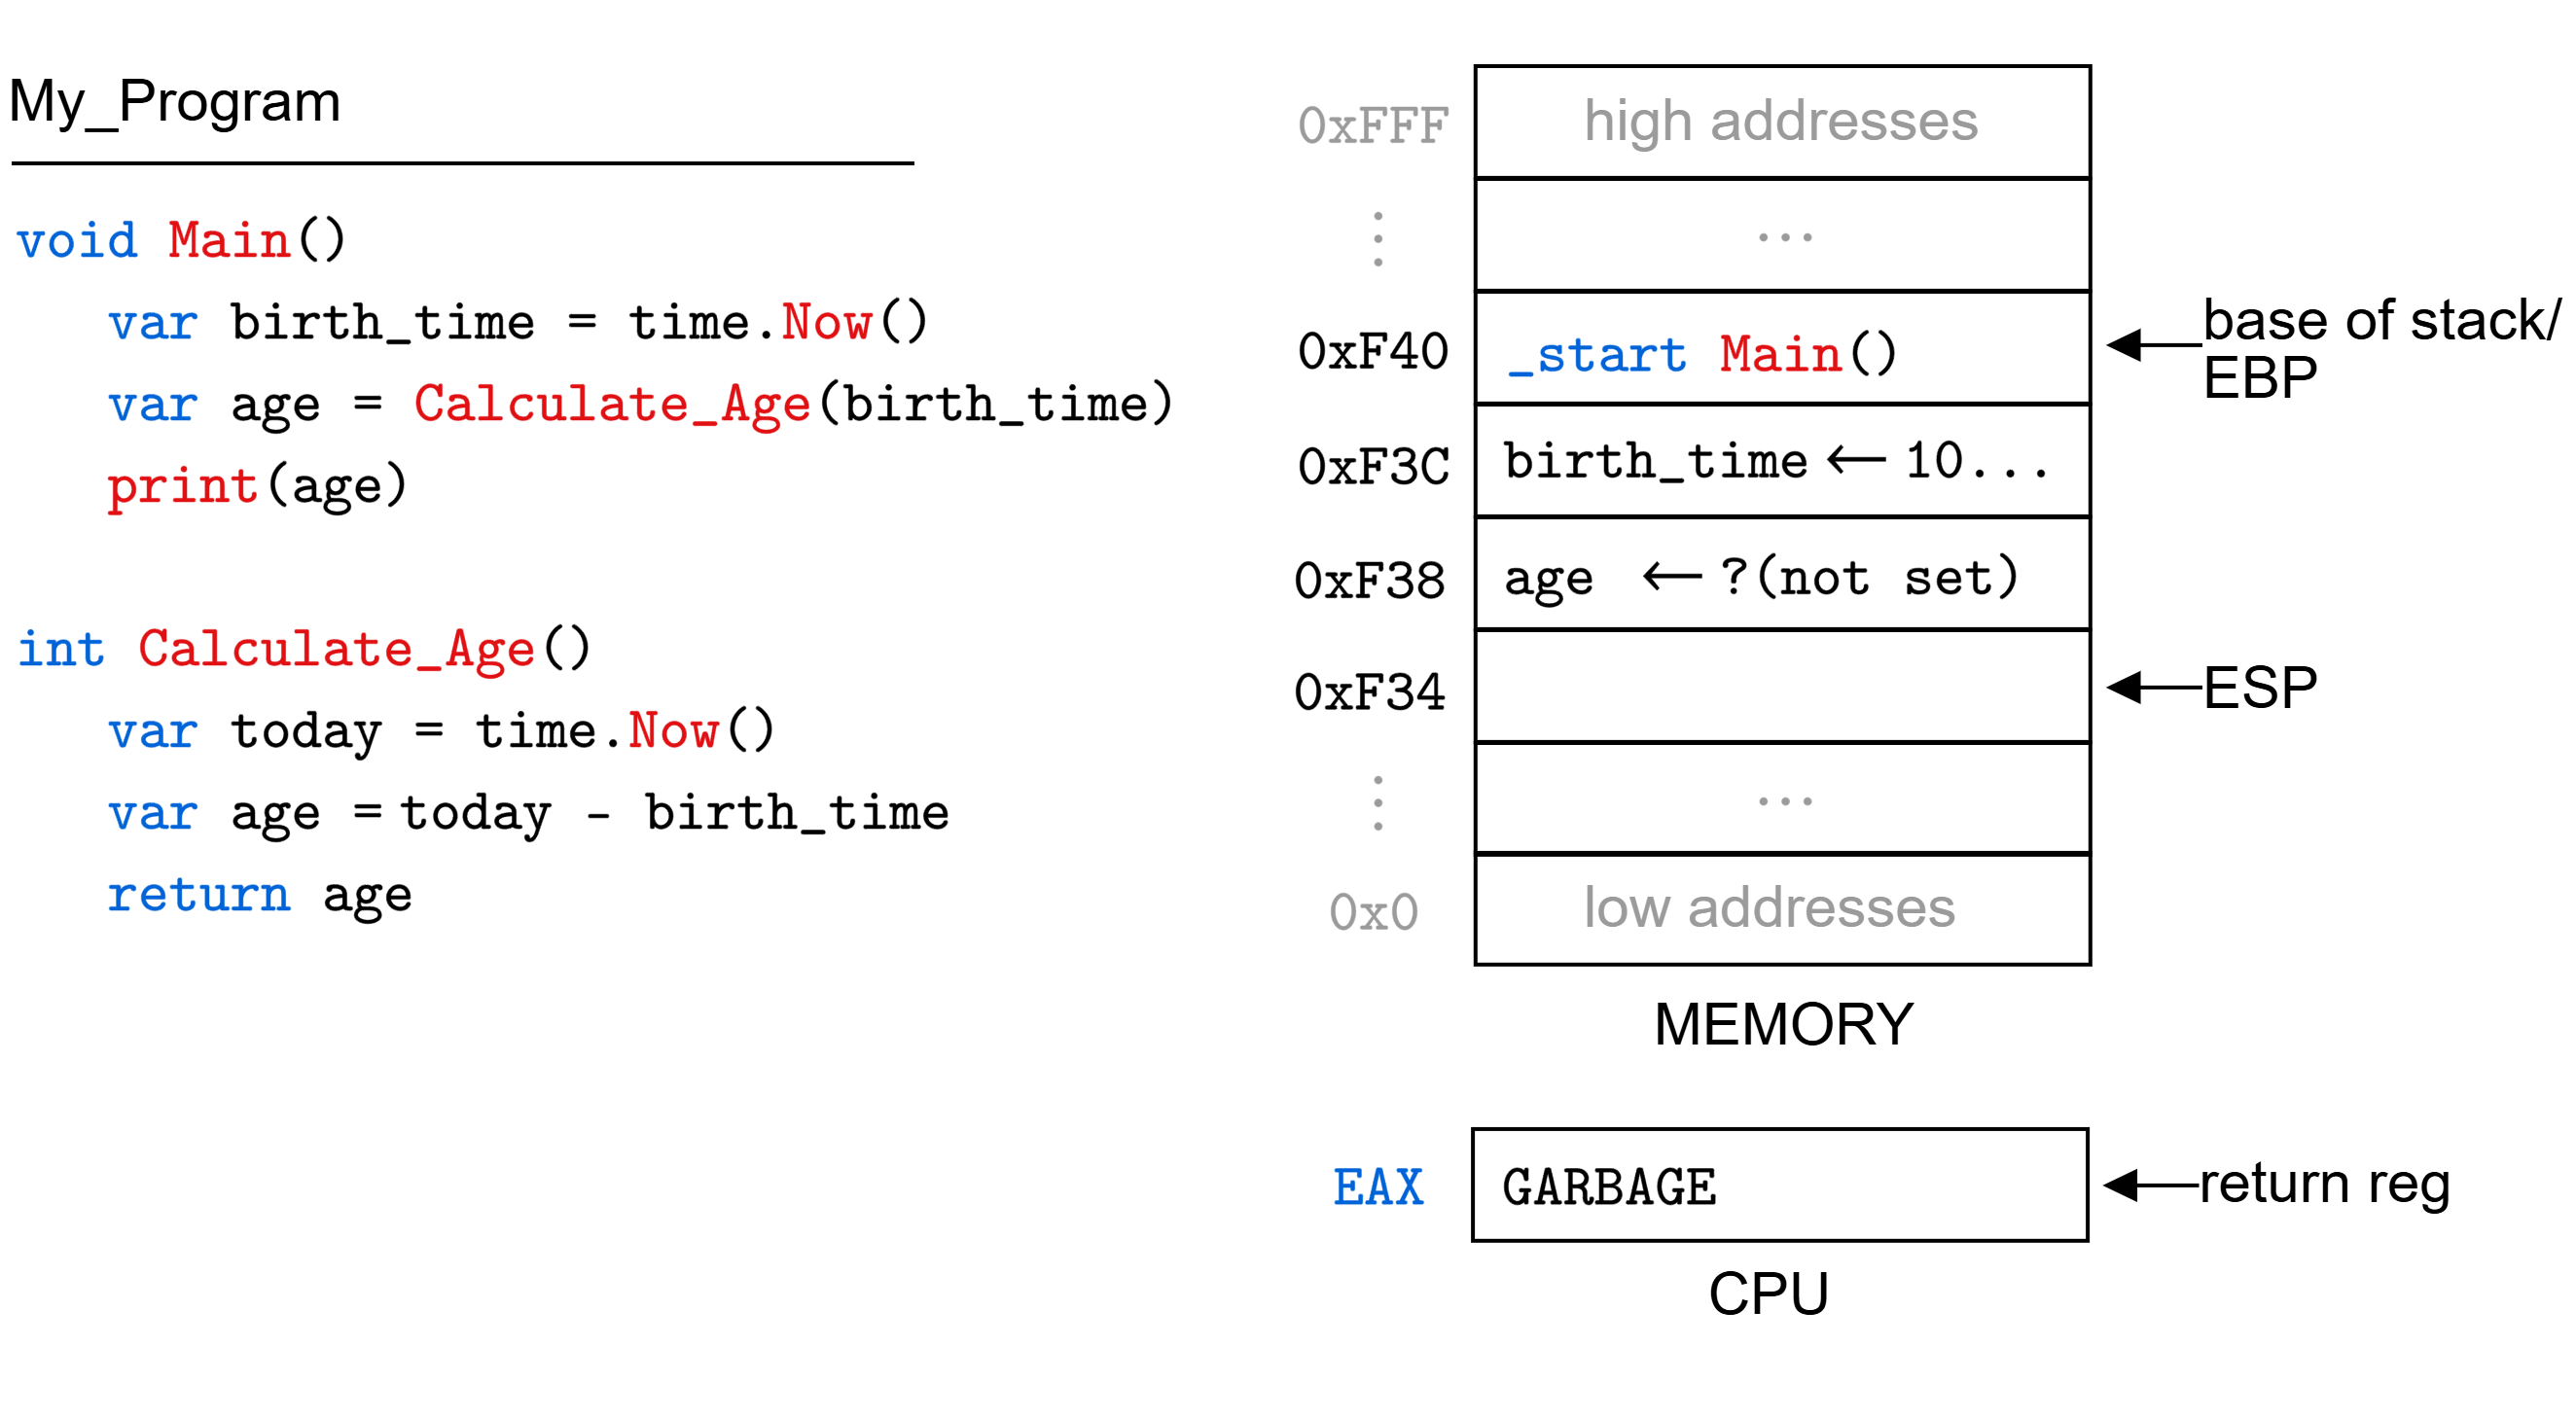
\includegraphics[width=\textwidth]{./Sections/stacks_heaps/call_stack_precise.png}
    \caption{Revisiting Figure (\ref{fig:call_stack}) with slight alterations to the code: This is a snapshot of the code executing right before \texttt{CalculateAge(birth\_time)} is called. For simplicity sake,
    let's say the stack begins at address \texttt{0xF40} (Hexadecimal), growing downwards. Here the base of the stack and the EBP are one and the same.
    We include the CPU's EAX (return register), which contains garbage. Address \texttt{0xF38} is currently just reserved space for `age'.}

\label{fig:call_stack_precise}
\end{figure}

\newpage 

\begin{figure}[!ht]
    \centering
    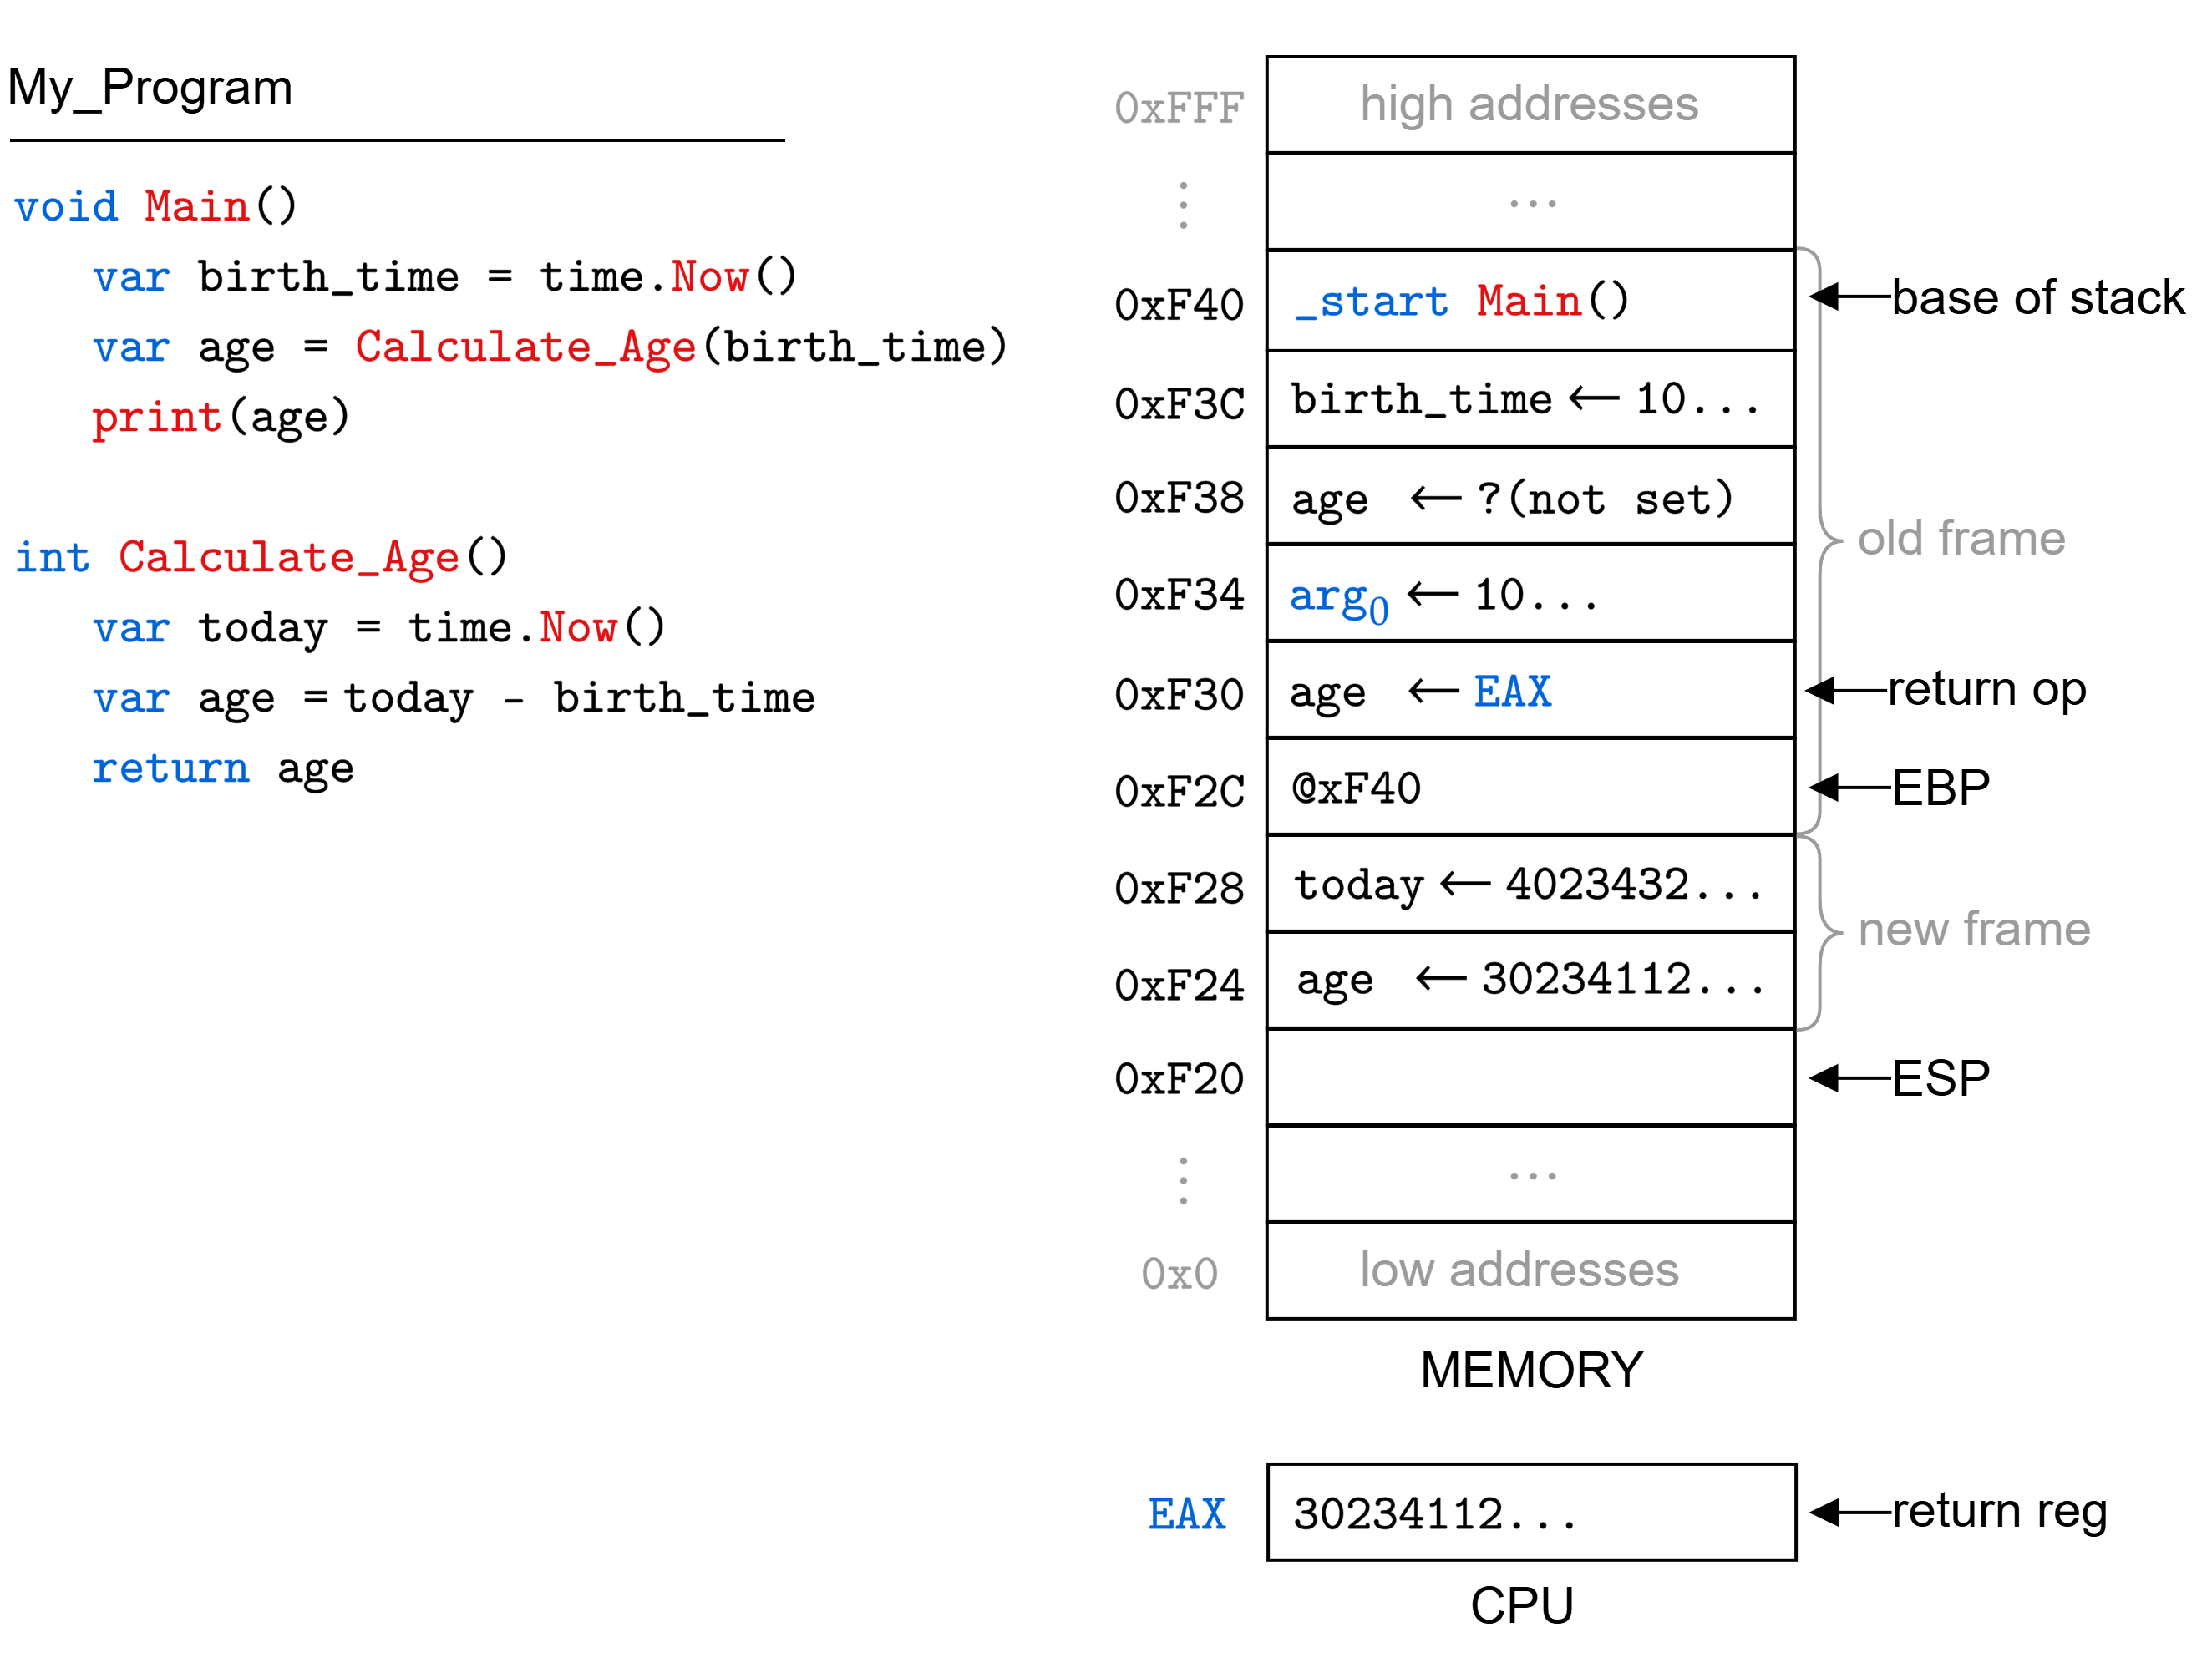
\includegraphics[width=\textwidth]{./Sections/stacks_heaps/call_stack_after.png}
    \caption{Revisiting Figure (\ref{fig:call_stack_precise}) at the moment the function \texttt{CalculateAge(birth\_time)} has supplied its return value to the EAX register, and is about to return.
    We see that before calling \texttt{CalculateAge(birth\_time)}: The old frame pushed it's arguments (\texttt{birth\_time}) onto the stack, then the return address (IP/Next Instruction) onto the stack,
    and finally the old EBP (Base Pointer) onto the stack. The `new frame' then sets the saved EBP address to the current EBP, concluding the old frame into the `new frame'. Moreover, since the offset
    looks for local variables below \texttt{0xF40}, the above `birth\_time' and `age' are \textbf{out of scope} for the `new frame', vice-versa. \textbf{Note:} This is 
    still a high-level absrtraction of what actually happens squentially with opcodes; Nonetheless, this is the fundemental idea of how a stack works. }
    \label{fig:call_stack_after}
\end{figure}

\noindent 
This concludes our discussion on stack structures; We continue with the heap structure next.
